\documentclass[a4paper,12pt,english]{report}

% Additional Packages
\usepackage{setspace}
\usepackage{pdflscape}
\usepackage{array}
\usepackage{hyperref}
\usepackage{booktabs}
\usepackage{ragged2e}
\usepackage{colortbl}
\usepackage{graphicx}
\usepackage{float}
\usepackage{longtable}
\usepackage{xcolor}
\usepackage[utf8]{inputenc}
\usepackage{babel}
\usepackage{amsmath}
\usepackage{times}
\usepackage{titlesec}
\usepackage[left=2.5cm, right=2.5cm, top=2.5cm, bottom=2cm]{geometry}

% Page setup
\renewcommand{\baselinestretch}{1.5}

% Title format

\begin{document}
% Title Page
\begin{titlepage}
  \centering
  \vspace*{\fill}
  
\includegraphics[width=100mm]{Logo rwu.png}\par
  \vspace{1cm}
  \Huge\textbf{Integration of 32-bit RISC-V ALU and ARM via Simple Bus with Scan Testability}\par
  \vspace{1cm}
  \Large{Masters in Electrical Engineering and Embedded Systems}\\
   \vspace{1cm}
  \Large\textbf{Authors}\par
  \Large{Tsedalu Fentaw Mekonen}\\
  \small{10841375}\\
  \Large{Nishanth Lazar Mohan }\\
  \small{15541744}\\
   \Large{Omkar Nimith Muthabyraiah }\\
  \small{16841822}\\       
\Large{Jayant Patil}\\
  \small{18041745}\\ 
 \Large{ Tejaswi Satish }\\
  \small{22041551}\\ 
  \vspace{0.5cm}
  \Large\textbf{Under the guidance of}\\
  \Large{Prof. Dr. Andreas Siggelkow}
  \vspace{0.5cm}
  \vspace*{\fill}
\end{titlepage}

\begin{table}[H]
    \centering
    \begin{tabular}{|c|c|p{3.5cm}|}
        \hline
        \multicolumn{3}{|c|}{\textbf{History Table}}\\
        \hline
        \multicolumn{3}{|c|}{Current Version: 2.0, 2024-01-16}\\
        \multicolumn{3}{|c|}{Previous Version: 1.0, 2023-10-30}\\
        \hline
        Paragraph (in previous version) & Paragraph (in current version) & Changes \\
        \hline
        - & All Chapters & Chapters created for the first time. \\
        \hline
    \end{tabular}
    \caption{History Table}
\end{table}

% Table of Contents
\tableofcontents
\newpage


\listoftables 
\newpage

% List of Figures
\listoffigures
\newpage
\chapter{Requirements}
\label{sec:requirements}

\newcolumntype{L}[1]{>{\raggedright\let\newline\\\arraybackslash\hspace{0pt}}m{#1}}
\newcolumntype{C}[1]{>{\centering\let\newline\\\arraybackslash\hspace{0pt}}m{#1}}
\newcolumntype{R}[1]{>{\raggedleft\let\newline\\\arraybackslash\hspace{0pt}}m{#1}}

\begin{center}
    \small % Reduce font size
    \begin{longtable}{|p{2.5cm}|p{1.5cm}|p{1.5cm}|p{4cm}|p{5.5cm}|}
    \hline
    \textbf{Requirements} & \textbf{ID} & \textbf{Priority} & \textbf{Verification} & \textbf{Description} \\ \hline
\textbf{General} & ~ & ~ & ~ & ~ \\ \hline
Peripheral & G1 & High & System C/ Simulation & The peripheral shall consist of  32-bit registers. 
 \\ \hline
 Read operation & G1 & High & System C/ Simulation & ALU must be readable via registers.
 \\ \hline
Write operation & G1 & High & System C/ Simulation & ALU must be writable via registers.
 \\ \hline
LEDs & G2 & High & System C/ Simulation & The LEDs should respond to logic high and low inputs. \\ \hline
Switches & G3 & High & System C/ Simulation & The switches should have high and low states, which can be updated by user inputs. \\ \hline
TAP Controller & G4 & High & System C/ Simulation & The TAP controller allows the movement of data through operations "Scan in" and "Scan out" via TDI and TDO pins respectively. It also allows the performance of a scan test. \\ \hline
\textbf{Communication} & ~ & ~ & ~ & ~ \\ \hline
Protocol: Simple bus & C1 & High & System C/ Simulation & The connection between the ARM core and the registers shall be established using the Simple bus.
 \\ \hline
\textbf{Software} & ~ & ~ & ~ & ~ \\ \hline
System C & S2 & High & N/A & The peripheral must be accurately modeled using System C.
 \\ \hline
\textbf{Test} & ~ & ~ & ~ & ~ \\ \hline
Scan Test & T1 & High & System C/ Simulation & Ensure a scan test implementation on registers with a scan chain model. \\ \hline
\end{longtable}
\end{center}


\chapter{Product Overview}

    
\section{Top Level View}
\subsection{Introduction}

The product overview that follows includes a detailed description of a project targeted at improving the capabilities of the ARM core on the Zed Board FPGA. The project entails the addition of a peripheral that includes a 32-bit RISC-V ALU that can be used for both reading and writing tasks. The registers are intended to control the LEDs by capturing switch inputs. The Simple bus facilitates communication between the ARM and the ALU. A TAP-controller (intended) and a scan chain are added into the system to assure the design's testability.

\begin{figure}[h!]
  \centering
  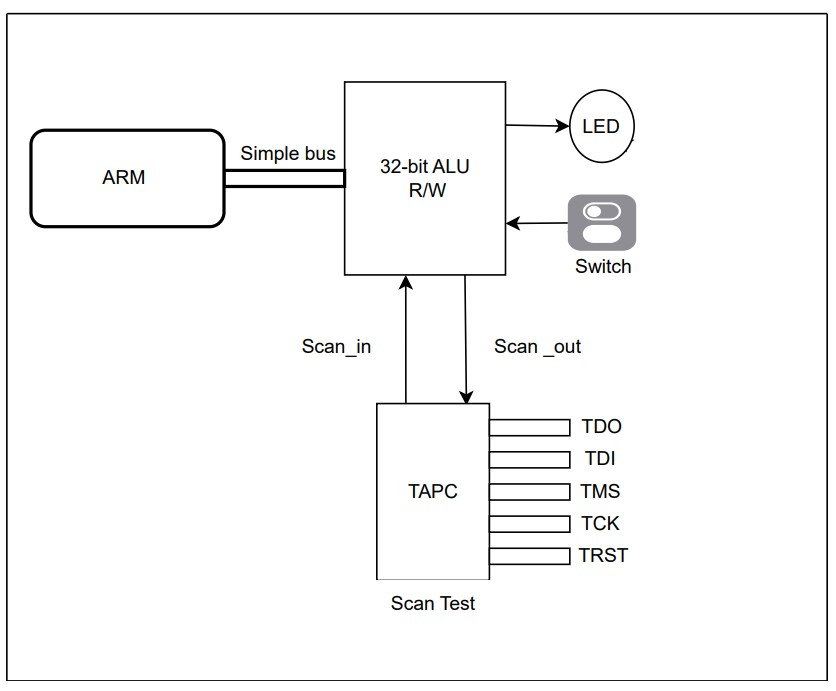
\includegraphics[width=0.7\linewidth]{FBD.jpg}
  \caption{Top Level view}
  \label{ref:TLV}
\end{figure}

As shown in the Figure \ref{ref:TLV}, we drive the LEDs by reading the states of the switches embedded on the ZedBoard. To enable the read and write operations, we develop a write function and a read function within the software component of the project. In addition, we implement 32 bit RISC-V ALU with System C. The code for the peripheral's 32-bit RISC-V ALU is meticulously crafted to facilitate both read and write operations, enabling seamless communication with the ARM core. One of the registers shall drive the LEDs, and the other shall receive inputs from switches on the ZedBoard. The communication between the ARM core and the ALU is established through the utilization of the Simple bus. Finally, to facilitate the testing of the system, it is intended to implement TAP controller, which enables the movement of data through the "Scan in" and "Scan out" operations via the TDI and TDO pins, respectively, and it also allows the execution of a scan test. 

\subsection{Key Features}
 \item \textbf {ARM}
\begin{itemize}
  The ARM system employs registers to store and manage data. Registers act as fast, accessible
storage units directly connected to the ALU. The code indicates that the ARM writes data to
specific registers, initiating the processing cycle. This implies a register-based architecture, a
common feature in many processor designs.
 \end{itemize}
   \item \textbf{RISC V 32-bit ALU}
  \begin{itemize}
    \item Reduced Instruction Set: The RISC-V ALU would support a reduced set of simple and efficient instructions, which are designed to execute quickly and enable faster processing.
    \item Single Clock Cycle Execution: Most instructions would be designed to execute in a single clock cycle, ensuring fast and efficient processing.
    \item Data Processing: The ALU operates on 32-bit data, which means it can perform arithmetic and logical operations on 32-bit binary numbers.
  \end{itemize}
  \item \textbf{Simple Bus}
  \begin{itemize}
    \item Supports read and write data transfers of 32-bit width.
    \item Supports Addressing and Identification.
    \item Error Handling and Correction.
    \item Synchronous bus systems for precise timing of data transfer.
  \end{itemize}
   \item \textbf {TAP Controller}
  \begin{itemize}
 
    \item IEEE Standard 1149.1
    \item 16-state Finite State Machine
    \item TAPC is part of JTAG
  \end{itemize}
  
   \item \textbf {Scan Chain}
  \begin{itemize}
 
    \item IEEE Standard 1149.1
    \item Ability to scan and test every flipflop in an Integrated Circuit (IC)
    \item Interconnect testing, In-System programming and debugging
  \end{itemize}
\newpage
\subsection{Functional Block Diagram}
The below depicted model will be actively implemented for the purpose of executing RISC-V Instructions on a Zybo board via ALU with 32-bit registers. These Registers are Readable and Writeable by the Processing System of the Zybo board via Simple bus. 
\vspace{2mm}

\textbf {Top Module:}
The Top module system's components, which include the ARM core, registers, ALU, and scan chain, communicate via a simple bus architecture. This design promotes efficient data sharing. The system stores data in registers, which are directly coupled to the ALU in a register-based design. The ALU conducts arithmetic and logical operations on data from registers, generating results that are returned to registers.
Write operations include beginning data writes to certain registers, delivering opcode to decide ALU operations, and carrying out the desired operation. Read operations involve getting results from specific registers and reading flags indicating various circumstances such as zero and carry flags, which provide information about the ALU's status following the operation.
\vspace{2mm}

\textbf {Simple Bus: }
 In a system, a fundamental communication framework is established through a simple bus architecture featuring master and slave components. This bus, functioning as a data highway, consists of parallel wires that convey signals such as data, addresses, and control instructions. At the forefront is the master, typically the central processing unit (CPU), which directs communication by generating control signals and addresses. Masters, typically CPUs, initiate read or write operations with specific slave devices.
\vspace{2mm}

\textbf {Scan Chain:}
 The design includes debugger and 7 registers of 32-bit each. The data transmission considered is Parallel In Parallel Out (PIPO). During the test mode, 1-bit Test Data Input (TDI) is fed to each register to the LSB position. The register being 32-bit, TDI is then left shifted to MSB and Test Data Output (TDO) is fetched from each of the register's MSB position. As TAPC is not part of the implementation, standalone debugger is used to pass the TDI.

\begin{figure}[h!]
  \centering
  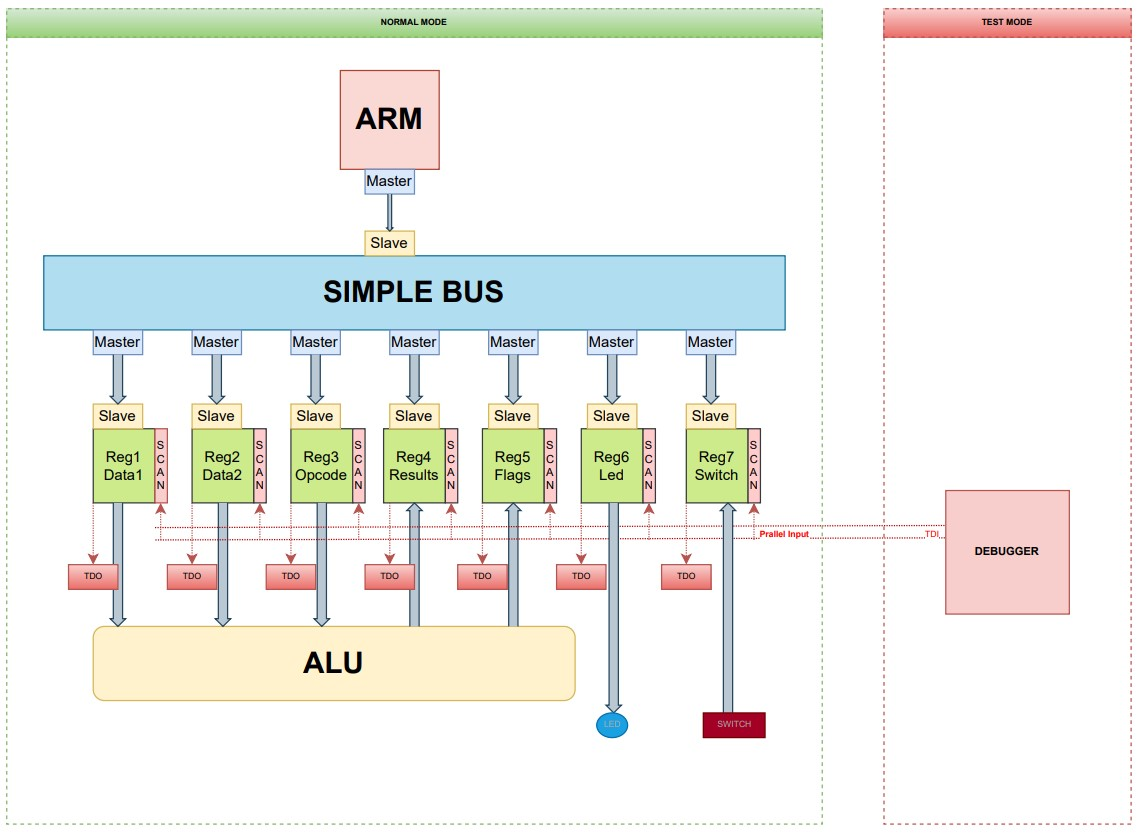
\includegraphics[width=18cm, height=16cm]{F_blockdiagram.jpg}
  \caption{Functional Block diagram}
  \label{fig:fbd}
\end{figure}

\chapter{Architecture Concepts}

\section{Bus Concept}
In a computing system, the orchestration of data transfers and communications on the bus is facilitated through the bus peripheral interface (BPI). This interface serves as a dedicated module responsible for managing interactions between the central processing unit (CPU), memory, and various peripheral devices connected to the system's bus. The crucial aspect highlighted in the statement is that the handling of bus transactions is not hardwired but is instead programmed. This programming aspect implies that developers write code to instruct the BPI on how to execute specific actions related to the bus, such as read and write operations, data transfers, and adherence to communication protocols. By utilizing programming instructions within the BPI, the system gains flexibility, allowing for customization of bus behavior to meet diverse requirements and adapt to various scenarios.
\subsection{Master BPI}
\begin{figure}[h!]
\centering
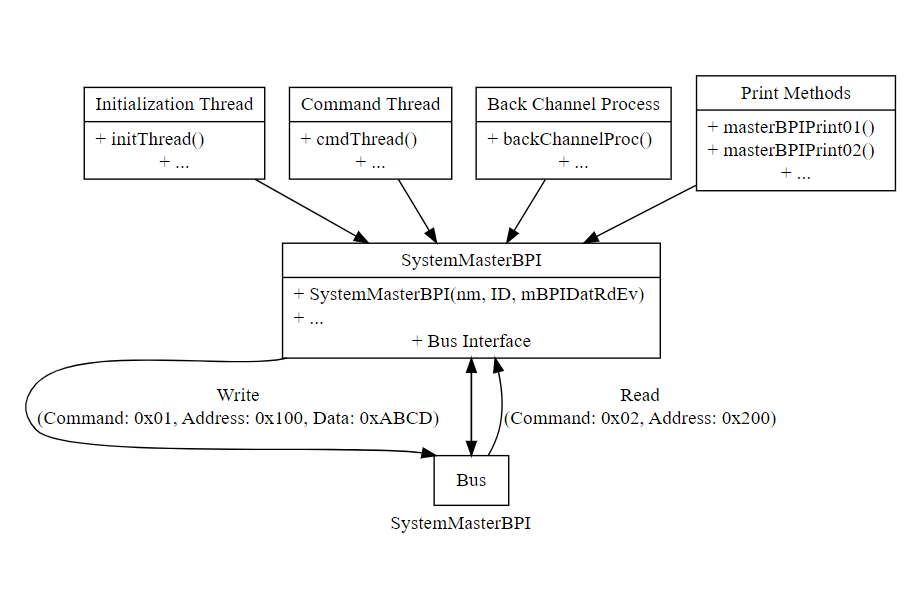
\includegraphics[width=18cm, height=10cm]{Master BPI.png}
\caption{Master BPI Block Diagram}
\end{figure}

\begin{itemize}
\item \texttt{SystemMasterBPI\textless T\textgreater} is a templated class that represents a System Master Bus and Peripheral Interface.
\item The constructor takes parameters such as the module name (nm), an ID, and a reference to an event (mBPIDatRdEv).
\item Initialization of the constructor includes setting up the module name, ID, event reference, and creating a socket (Master1Socket).
\item Two SystemC threads (initThread and cmdThread) are registered in the constructor.
\item Input exports (\texttt{data\textunderscore i}, \texttt{write\textunderscore i}, \texttt{address\textunderscore i}) are bound to corresponding internal signals (\texttt{dataWr\textunderscore s}, \texttt{write\textunderscore s}, \texttt{address\textunderscore s}).
\end{itemize}
\textbf{Initialization Thread:} 
\begin{itemize}
\item \texttt{initThread} is a SystemC thread responsible for controlling the bus transactions. It waits for changes on the bus (\texttt{cmd\textunderscore e} event) and reacts accordingly.

    \item If a write command is detected, it retrieves data from \texttt{dataWr\textunderscore s} and prepares a payload for the socket. The payload is sent to the socket using blocking transport (\texttt{b\textunderscore transport}).

    \item If a read command is detected, it processes the read data, writes it to \texttt{data\textunderscore o}, and notifies the associated event (\texttt{mBPIDatRdEv\textunderscore e}).

    \item Back channel responses are checked for errors using \texttt{backChannelProc}.

    \item Additional printouts are included for debugging purposes.

    \item There's a wait for a delay at the end.
\end{itemize}

\textbf{Back Channel Process:}
\begin{itemize}
\item \texttt{backChannelProc} is responsible for processing back-channel responses from the socket.

    \item If there is a response error, it reports the error using \texttt{SC\textunderscore REPORT\textunderscore ERROR}.

    \item If there is no error, it processes the successful response.

    \item If debug prints are enabled, it prints relevant information.
\end{itemize}

\textbf{Command Thread:} 
\begin{itemize}
\item \texttt{cmdThread} is another SystemC thread responsible for monitoring changes in the write signal (\texttt{write\textunderscore s}).

\item It waits for the signal to change and then notifies \texttt{initThread} that something has happened on the bus.
\end{itemize}

\textbf {masterBPI Print Methods}
\begin{itemize}
\item \texttt {masterBPIPrint01} This method prints a message indicating that the Master-BPI module is waiting for some action on the bus.
\item \texttt {masterBPIPrint02} Prints a message indicating the end of waiting for action on the bus.
\item \texttt {masterBPIPrint03} Prints information about a bus operation, including the byte address, data, and command (Read or Write).
\item \texttt {masterBPIPrint04} Prints a message indicating the end of a delay in the bus operation.
\item \texttt {masterBPIPrint05} Prints information about a successful back-channel response, including the data received.
\item \texttt {masterBPIPrint06} Prints information about a change in the command signal on the bus.
\end{itemize}
\newpage
\subsection{Slave BPI}
\begin{figure}[h!]
\centering
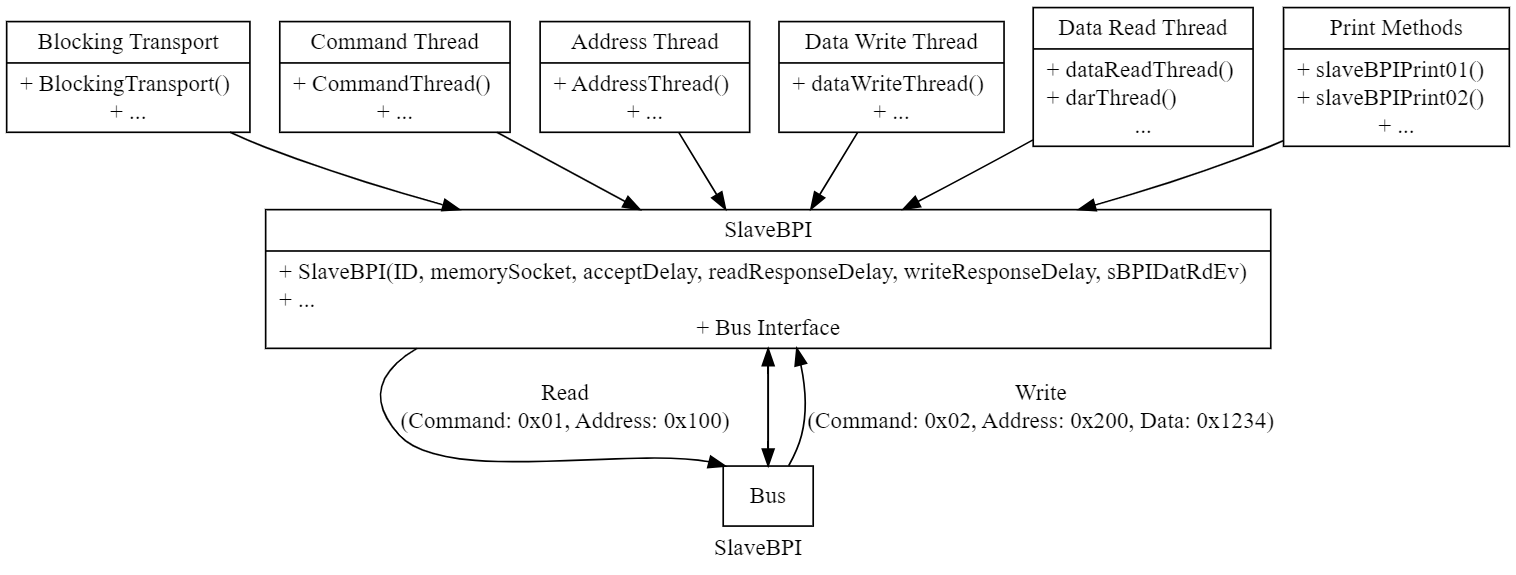
\includegraphics[width=0.8\linewidth]{graphviz.png} % Adjust the width as needed
\caption{Slave BPI Block Diagram}
\end{figure}

\textbf{Components:}
\begin{itemize}
    \item \texttt{ID}: Target ID for the slave device.
    \item \texttt{memorySocket}: Socket name for communication.
    \item \texttt{acceptDelay}: Accept delay for bus transactions.
    \item \texttt{readResponseDelay}: Delay for read response.
    \item \texttt{writeResponseDelay}: Delay for write response.
    \item \texttt{sBPIDatRdEv}: Reference to an event used for data read .synchronization
\end{itemize}

\textbf{Blocking Transport Method:}
\begin{itemize}
    \item Implements the TLM blocking transport method for handling read and write transactions.
    \item Extracts information from the payload, such as command, address, data pointer, length, etc.
    \item Checks for errors (address error, byte enable error, burst error).
    \item Performs read or write operations based on the command.
    \item Sets the response status and delay accordingly.
\end{itemize}

\textbf{Command Thread:}
\begin{itemize}
    \item Delivers "Read" or "Write" signals to the \texttt{sc\textunderscore export}.
    \item Monitors changes in the \texttt{write\textunderscore s} signal and writes the value to the \texttt{write\textunderscore o} \texttt{sc\textunderscore export}.
\end{itemize}

\textbf{Address Thread:}
\begin{itemize}
    \item Delivers/writes "Address" signals to the \texttt{sc\textunderscore export}.
    \item Monitors changes in the \texttt{adr\textunderscore s} signal and writes the value to the \texttt{address\textunderscore o} \texttt{sc\textunderscore export}.
\end{itemize}

\textbf{dawThread:}
\begin{itemize}
    \item Delivers/writes "Data" signals to the \texttt{sc\textunderscore export}.
    \item Monitors changes in the \texttt{daw\textunderscore s} signal and writes the value to the \texttt{data\textunderscore o} \texttt{sc\textunderscore export}.
\end{itemize}

\textbf{darThread:}
\begin{itemize}
    \item Handles data read events and triggers the bus transport.
    \item Waits for data coming from the functional block (\texttt{sBPIDatRdEv\textunderscore e}).
    \item Reads data from the \texttt{dataRd\textunderscore s} signal.
    \item Notifies the bus transport that data is available (\texttt{dataRd\textunderscore e.notify(SC\textunderscore ZERO\textunderscore TIME)}).
\end{itemize}


\textbf{SlaveBPI Print Methods:}
\begin{itemize}
    \item \texttt{slaveBPIPrint01} - Prints information about a \texttt{b\textunderscore transport} operation, including the word address, maximum memory size, and target ID.
    \item \texttt{slaveBPIPrint02} - Prints information about a read operation, including the word address and data.
    \item \texttt{slaveBPIPrint03} - Prints information about a write operation, including the word address and data.
    \item \texttt{slaveBPIPrint04} - Prints information about an ignore command, including the word address, data, and command.
    \item \texttt{slaveBPIPrint05} - Prints information about a data read event from the functional block.
\end{itemize}

\section{Registers}


A 32-bit RISC-V register serves as a dedicated storage location within a computer's central processing unit (CPU), designed to accommodate a 32-bit binary value. The term ``32-bit'' denotes the register's capacity, indicating its ability to store data comprising 32 binary digits (bits). Integral to the RISC-V architecture, these registers form part of the general-purpose register set employed by the CPU for various computational tasks.Key attributes of a 32-bit RISC-V register encompass its size, capable of holding 32 bits, offering a vast range of $2^{32}$ potential binary combinations. These registers are designated as general-purpose, allowing them to store diverse data types, including integers, addresses, and other fundamental data entities. Embedded within the RISC-V architecture, denoting Reduced Instruction Set Computing - Version 5, these registers play a pivotal role in storing and manipulating data during the execution of instructions.

Beyond their general-purpose nature, 32-bit RISC-V registers contribute significantly to data processing tasks, participating in arithmetic and logical operations. The CPU utilizes these registers to perform computations on the stored data, underscoring their indispensability in executing a wide array of tasks and programs. The addressing of RISC-V registers involves distinct register names, such as \texttt{x0, x1, ..., x31}, providing a systematic means to identify and manage different registers within the processor.Programmers and compilers leverage the capabilities of these registers to optimize code execution, capitalizing on the simplicity and efficiency inherent in the RISC-V architecture. The preference for 32-bit registers in modern computer architectures reflects a strategic balance between computational capabilities and memory efficiency, affirming their central role in contemporary computing systems.

\section{ARM System Architecture Overview}


The ARM system relies on a simple bus architecture for communication between different components. The bus facilitates the transfer of data between the ARM core, registers, ALU, and memory. This straightforward communication scheme simplifies the overall design and ensures efficient data exchange.
\subsection{ Register Interaction:}
 The ARM system employs registers to store and manage data. Registers act as fast, accessible storage units directly connected to the ALU. The code indicates that the ARM writes data to specific registers, initiating the processing cycle. This implies a register-based architecture, a common feature in many processor designs.
 \subsection{ALU Operation:}
 The Arithmetic Logic Unit (ALU) is a critical component of the ARM system responsible for performing arithmetic and logical operations on data. The ALU takes input data from registers, executes the specified operation (such as addition, subtraction, etc.), and produces a result. The result is then stored back into registers for further processing or retrieval.

\subsection{Write Operations}

\begin{enumerate}
    \item \textbf{Operand Data Write (Write Section)}: The ARM system initiates write operations by providing operand data to specific registers. This is done through the simple bus, where data is written to designated registers with unique identifiers (Slave IDs).


   \item\textbf{Opcode Write}: The ARM system also writes opcode to a specific register. This opcode determines the type of operation the ALU should perform. The control signal is transmitted over the bus and stored in the corresponding register.

   \item\textbf{ALU Processing}: Once the necessary data and opcode are in place, the ALU executes the specified operation. This involves reading data from the registers, performing the operation, and generating a result.
\end{enumerate}

\subsection{Read Operations} 

1. \textbf{Result Read (Read Section)}: After the ALU completes the operation, the result is stored in a designated register. The ARM system then reads this result from the register, providing visibility into the outcome of the computation.\\
2. \textbf{Flag Read}: Additionally, the system reads flags that indicate various conditions such as zero flags, carry flags, etc. These flags provide information about the state of the ALU after the operation.

\section{Arithmetic Logic Unit (ALU)}
The brains of the computer are the arithmetic logic unit (ALU), which can execute logical operations like AND and OR as well as set less than instructions. It can also perform arithmetic operations like addition and subtraction. In order to demonstrate how combinational logic functions, this section builds an ALU using four hardware building blocks: AND and OR gates, inverters, and multiplexers. We'll see how more ingenious designs can speed up addition and subtraction. We require a 32-bit wide ALU since the RISC-V registers are 32 bits wide. The Arithmetic Logic Unit (ALU) plays a crucial role in the execution of operations within a computer's central processing unit (CPU). Once the essential data and control signals are properly configured, the ALU swings into action, carrying out the specified operation. This process encompasses the retrieval of necessary data from registers, the execution of the operation itself, and the subsequent generation of a resulting value.
\begin{table}[h]
	\centering
	\begin{tabular}{|l|l|l|}
		\hline
		Opcode in decimal & Opcode in Binary & ALU Operation \\
		\hline
		0 & 0000 & AND \\
		1 & 0001 & OR \\
		2 &0010 & Adder \\
		3 & 0011 & Subtract \\
		4 & 0100 & Set less than \\
		5 & 0101 & NOR \\
		\hline
  
	\end{tabular}
 \caption{The values of the three ALU control lines, Ainvert, Bnegate, and Operation, and the corresponding ALU operations}
\end{table}

As the ALU concludes its computation, the resulting value is securely stored in a designated register. This register acts as a temporary holding space for the outcome of the operation. Following this, the ARM system proceeds to read or fetch this result from the register. This step is pivotal for gaining visibility into the computed outcome and is fundamental to the overall functionality of the ALU.

Beyond obtaining the numerical result, the system also seeks information about the state of the ALU through the retrieval of flags. Flags serve as indicators that convey specific conditions met during the operation. These conditions may include whether the result is zero, if a carry occurred, or other relevant status updates. By reading these flags, the system gains valuable insights into the nuances of the computation, allowing for further analysis and decision-making in subsequent stages of processing. This aspect enhances the overall efficiency and adaptability of the ALU in responding to diverse computational scenarios.

\newpage
\section{Scan Chain}
 An illustration depicts the distinctions between a scannable and a standard flip-flop. The scannable flip-flop only interacts with the TDO pin, whereas the regular flip-flop connects to both the TDI and TDO pins. These flip-flops must be part of a scan chain in order to be tested effectively. The scan chain connects all flip-flops in a series loop; the TDO pin of one flip-flop is immediately connected to the TDI pin of the next flip-flop.  To load test vectors, scan chain clocks are pulsed after the TDI pins have been set to the required value. This process ensures that the test vector is systematically shifted along the scan chain before being loaded into the appropriate flip-flops. To unload a test vector, pulse the scan chain clock while setting the TDI pin to a high impedance condition. This smart action causes the test vector to go through the flip-flops and emerge on the TDO pin, completing the circuit's testing cycle.

 \begin{figure}[h!]
  \centering
  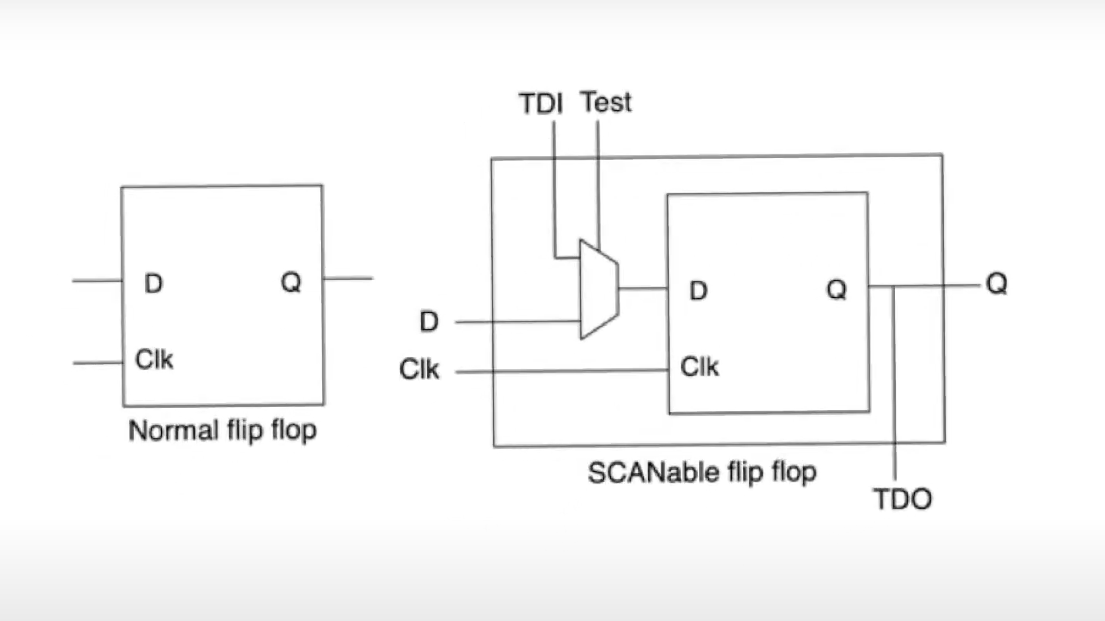
\includegraphics[width=0.7\linewidth]{scanff.png}
  \caption{Scan Flipflop}
\end{figure}

\chapter{Description of Design Elements}
\section{ARM}
\begin{enumerate}
    \item \textbf{Constructor:}
   - The constructor initializes the ARMFunc module and sets up its SC\textunderscore THREADs.
   - It also binds the data\textunderscore i port to the dataIn\textunderscore s export.
   \item \textbf{getDatThread:}
   - This thread waits for an event (mFuncDatRdEv\textunderscore e) signaling that read data is available.
   - Upon receiving the signal, it reads data from the dataIn\textunderscore s port and prints information if    specified.
   \item \textbf{armSequenceThread:}
   - This is the main algorithm of the ARMFunc module, executed in a SystemC SC\textunderscore THREAD.
   - It performs a series of write and read operations to simulate the behavior of an ARM processor.
   - The operations include writing data to operands, writing an opcode (control signal), and reading results and flags.
   - The printed information includes details about the operations, addresses, data values, and timing.
  \item \textbf{Flag Handling:}
The code includes flag handling, where different flags (such as zero, carryin, lessthan, carryoverflow, negative) are checked based on ALU operation results. Flags play a crucial role in controlling program flow and providing status information.
\item \textbf{armWrCmd and armWrAndPrint:}
   - armWrCmd writes data to the BPI (Bus-Peripheral Interface) by sending a write command.
   - armWrAndPrint additionally prints information about the write operation.

 \item \textbf{armRdCmd and armRdAndPrint:}
   - armRdCmd reads data from the BPI by sending a read command.
   - armRdAndPrint additionally prints information about the read operation.

  \item \textbf{armRd1Print, armWr1Print, armFuncPrint01:}
   - These functions are responsible for printing various information related to read and write operations. The code contains various print statements that provide detailed information about the execution of the ARM functional block, including read and write operations, addresses, data values, and timing information.
\end{enumerate}
 \begin{figure}[h!]
  \centering
  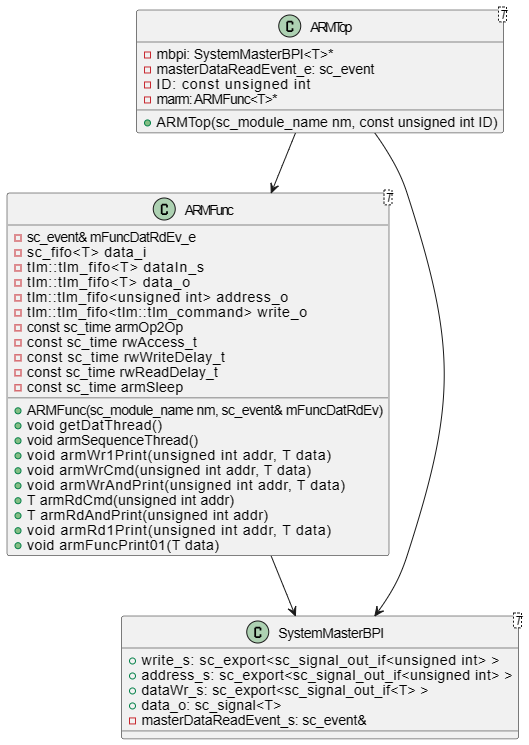
\includegraphics[width=0.7\linewidth]{arm.drawio.png}
  \caption{ARM Class Diagram}
\end{figure}

\section{Registers}
\subsection{Operation}

In this system architecture, the coordination of signals, crucial for the interaction between the master (simple bus), registers, and the 32-bit RISC-V ALU, is typically implemented through code. Signal binding in the code ensures that the correct signals are generated, transmitted, and interpreted by the respective components.

For instance, in a read operation, the code governing the master generates the appropriate read signal and addresses the specific 32-bit register on the bus. The code in the register then interprets this signal, fetching the requested data from the 32-bit ALU and placing it onto the bus for the master to read. Similarly, during a write operation, the code generates the write signal, transmits both the 32-bit data and the target register's address, and instructs the 32-bit ALU to store the incoming information in the designated register.

This code-driven signal binding ensures a synchronized and organized communication flow within the system. It aligns the actions of the master, registers, and the 32-bit RISC-V ALU, ensuring that data is transferred accurately and operations are executed as intended. The coded logic governing signal interactions forms a fundamental aspect of the system's functionality, contributing to its efficiency in data handling and computation.

\section{Simple Bus}
In a computer system, a simple bus architecture with master and slave components establishes a fundamental communication framework. The bus, akin to a data highway, comprises parallel wires conveying signals like data, addresses, and control instructions. At the helm is the master, typically the central processing unit (CPU), orchestrating communication by generating control signals and addresses. Masters initiate read or write operations with specific slave devices.
\vspace{2mm}

Slaves, encompassing peripherals, memory modules, or other subsystems, await commands from the master. Each slave is assigned a unique address. When the master desires data from a slave, it transmits the target address for a read operation, prompting the slave to respond with the requested data. Conversely, for a write operation, the master transmits both the target address and the data to be written, and the addressed slave stores the information in the appropriate location.

This interaction encapsulates the essence of a master-slave relationship on the bus, where the master takes charge of communication initiation, and slaves respond to these requests. Bus arbitration mechanisms ensure coordinated access, crucial in systems with multiple masters. Ultimately, this simple bus architecture facilitates the seamless exchange of data and instructions, forming the backbone of communication within a computer system.


\subsection{Simple Bus operation with Registers}
\begin{figure}[h!]
\centering
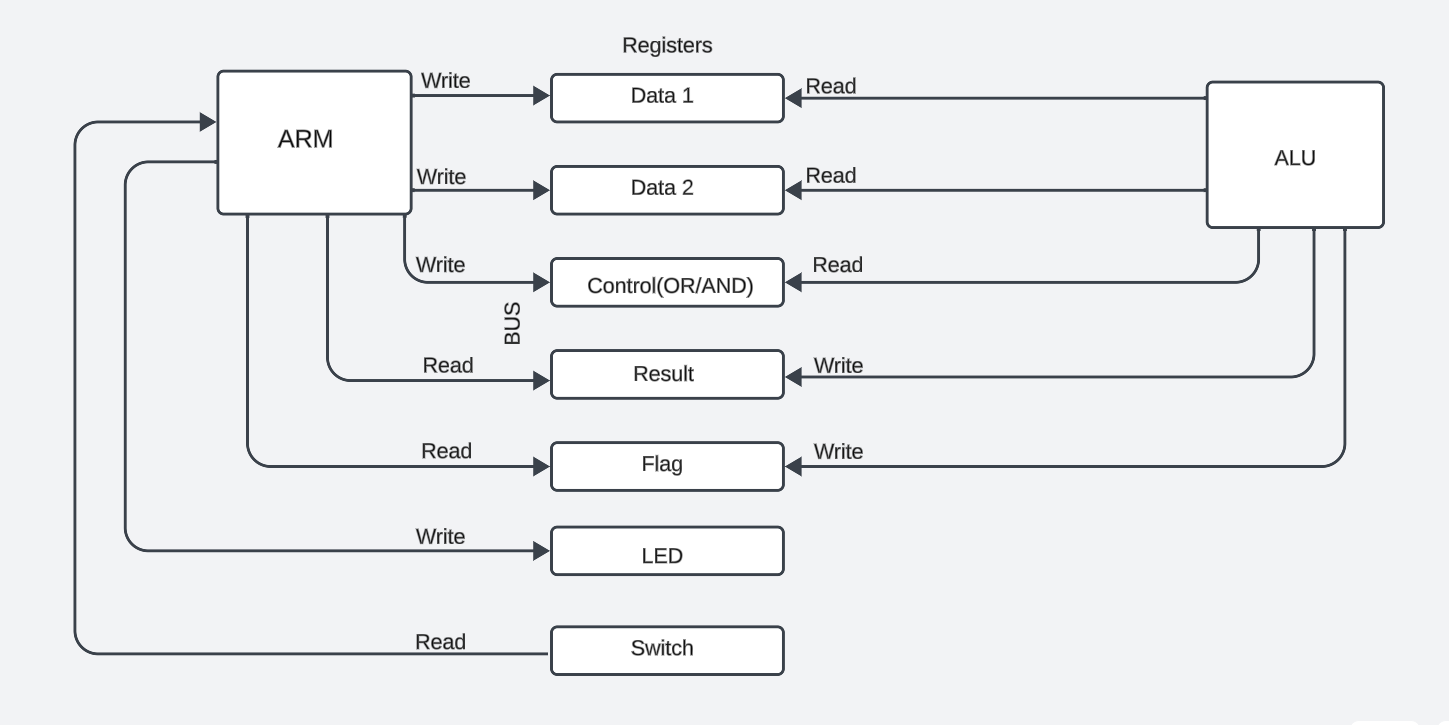
\includegraphics[width=16cm, height=14cm]{simple_bus.png} % Adjust the width as needed
\caption{Simple Bus Block Diagram}
\end{figure}
\newpage
In a system featuring a simple bus as the master connected to 7 registers functioning as slaves, a communication network is established to facilitate data transfer and control within the system. The simple bus, acting as the master, initiates and coordinates data transactions by sending control signals and addresses to communicate with the connected registers. Each of the 7 registers, serving as slaves, is assigned a unique address on the bus, enabling the master to target and interact with individual registers. Building upon the initial configuration of a simple bus connected to 7 registers, where registers 1 and 2 write data, register 3 writes control, register 4 reads results, register 5 reads flag conditions, and registers 6 and 7 are designated for an LED and a switch respectively, the system extends its functionality by further connecting these registers to ARM with Arithmetic Logic Unit (ALU).
\vspace{2mm}

The ALU, a digital circuit capable of performing arithmetic and logical operations, becomes an integral part of the system's computational capabilities. During operations involving data written to registers 1 and 2, the simple bus coordinates the transfer of this data to the ALU for computation. Register 3, responsible for control signals, communicates instructions to the ALU, directing it on the type of operation to be performed. After computations are executed within the ALU, the results are stored in register 4, which serves as a data reader. The flag conditions, read from register 5, can influence the ALU's operations or be used by the ARM to make decisions based on the system's state. The interconnected setup ensures a seamless flow of data and control between the registers and the ALU. Additionally, the integration of registers 6 and 7, associated with an LED and a switch respectively, allows the system to interact with external components. For instance, the switch state (register 7) might influence the ALU's behavior, and the results or status could be reflected through the LED (register 6). This comprehensive communication network, with registers playing specific roles and the ALU contributing computational capabilities, enhances the system's versatility and efficiency. The simple bus facilitates these interactions, creating a framework for data exchange, control, and computation within the system.
\newpage
\section{ALU}
 \begin{figure}[h]
	\centering
	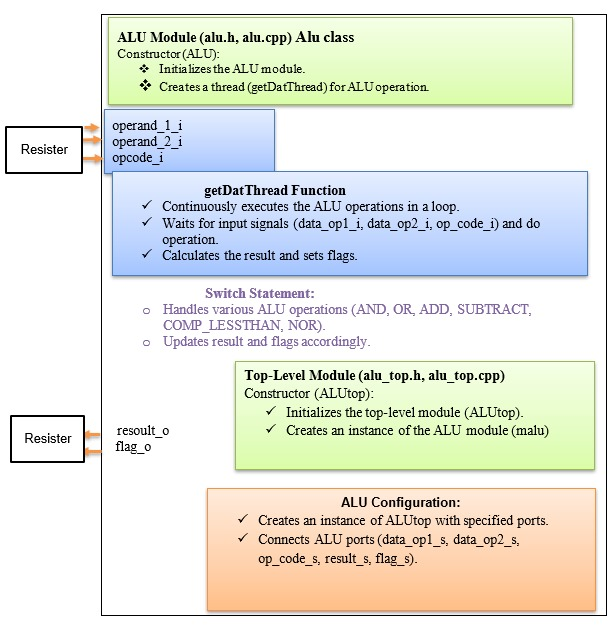
\includegraphics[width=0.9\textwidth]{ALU_class_d.jpg} % Adjust the filename as needed
	\caption{ALU Class Diagram.}
 \end{figure}
 
\subsection{A 1 Bit ALU  AND and OR}
The 1-bit logical unit for AND and OR is shown in Figure \ref{ref: 1bit and or}. Next, the multiplexer on the right takes the inputs from the ARM and performs the operation of operand\_1 AND operand\_2 or operand\_1 OR operand\_2, depending on whether the value of operation is 0 or 1. See how the control and output lines of the multiplexer have been renamed to reflect the function of the ALU more accurately.
 \begin{figure}[ht]
	\centering
	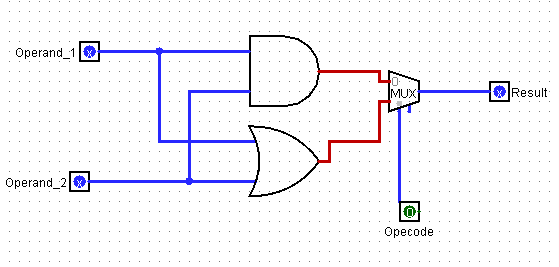
\includegraphics[width=0.6\textwidth]{and_or} % Adjust the filename as needed
	\caption{The 1-bit logical unit for AND and OR.}
	\label{ref: 1bit and or}
\end{figure}
\subsection{Addition and Subtraction}
Addition and subtraction are the next function to be included. Two operand inputs and a single-bit output for the sum and difference are required for an adder and subtractor. To pass on the carry, a second output known as CarryOut is required. We require a third input because the CarryOut from the neighbor adder needs to be included as an input. CarryIn is the name of this input.\\
Adders carry out subtraction in the same way as they would add the negative form of an operand. Remember that we can quickly negate a two's complement number by adding 1 and inverting each bit, which is also referred to as the one's complement. The inputs and outputs of a 1-bit adder and subtractor are displayed in Figure \ref{ref: 1bit and}.
 \begin{figure}[ht]
	\centering
	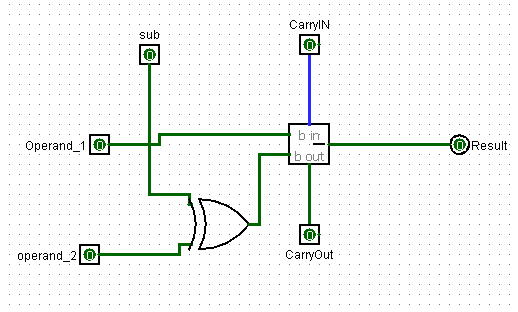
\includegraphics[width=0.6\textwidth]{add_sub} % Adjust the filename as needed
	\caption{The 1-bit Addition and subtraction}
	\label{ref: 1bit and}
	\end{figure}
 \newpage
	\subsection{1-Bit ALU}
Figure\ref{ref: set less than} [ref 1, page1187 ] below illustrates how we compiled all of the individual AND, OR, and addition operations into a single 1-bit ALU operation after completing each one separately. Furthermore, to these three operations—add, AND and OR we need set less than instruction of RISC-V ALU for comparing of the two operands that we have taken from the ARM.
so, the set less than instruction (slt) Recall that the operation produces 1 if rs1  less than rs2, and 0 otherwise.
 \begin{figure}[ht]
	\centering
	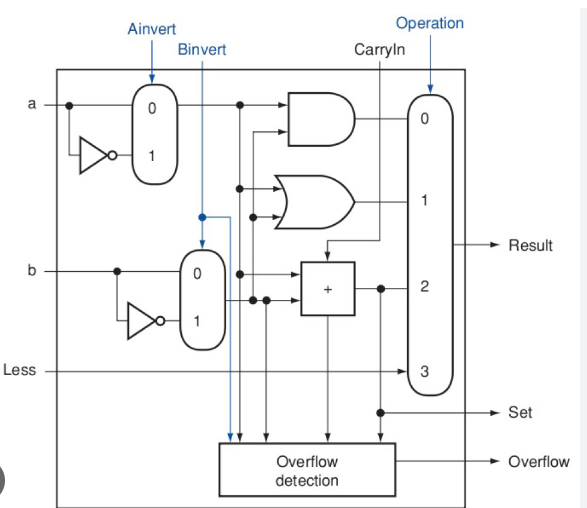
\includegraphics[width=14cm, height=12cm]{1bit alu} % Adjust the filename as needed
	\caption{A 1-bit ALU }
	\label{ref: set less than}
\end{figure}
\newpage
	\subsection{A 32 Bit ALU Operation}
Once the 1-bit ALU is complete, we connect the adjacent "boxes" to generate the complete 32-bit ALU, which can be used for addition, subtraction, AND, OR, and set less than input. After performing the subtraction operation as follows, a–b, CarryIn and Binvert are now both set to 1. Both control lines ought to be zero in the case of additions or logical operations. Therefore, as illustrated in Figure \ref{ref: 32 bit}[ref 1, page1191 ], we can simplify the control of the ALU by combining the CarryIn and Binvert into a single control line known as Bnegate.
 \begin{figure}[ht]
	\centering
	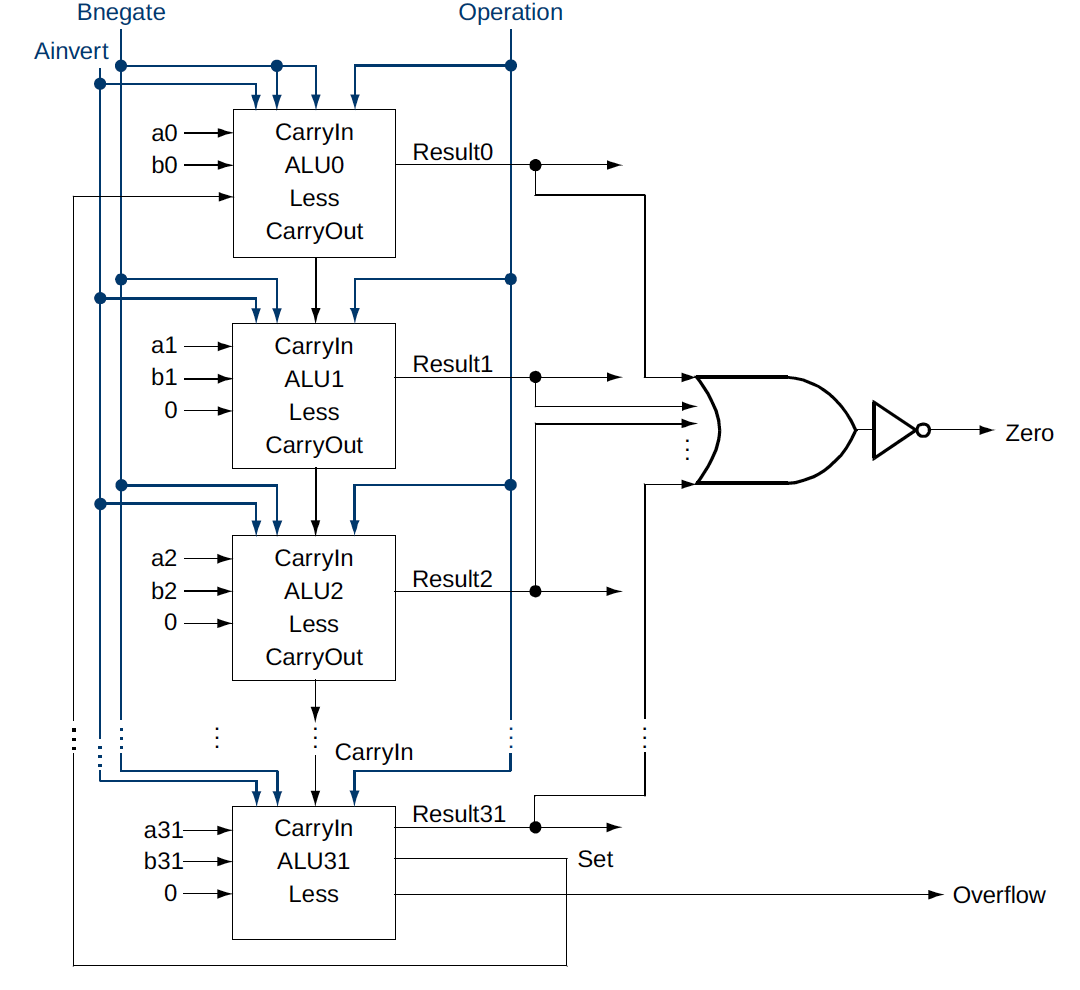
\includegraphics[width=14cm, height=14cm]{32bitalu} % Adjust the filename as needed
	\caption{The final 32 bit ALU}
	\label{ref: 32 bit}
\end{figure}
\section{Scan Chain}
TLM (Transaction Level Modeling) based system is used that simulates a master (scanchainFunc) interacting with a System Master BPI (Bus and Peripheral Interface) module (SystemMasterBPI) and a stimulus module (Stim).

\begin{enumerate}
    \item scanchainFunc:

\begin{itemize}
    \item A templated class representing the functionality of a master in a scan chain system.

    \item The getDatThread thread waits for the read data event (mFuncDatRdEve) and then notifies the algorithm about the availability of data.

    \item The scanchainSequenceThread thread executes a scan chain sequence involving writing data to multiple registers and printing the results.

    \item The sequence involves writing data to multiple registers (Reg1, Reg2, Reg3, Reg4, Reg5 ) with slave ID's corresponding to each register and printing the results.

    \item It has methods for printing, writing, and reading data from the System Master BPI.
\end{itemize}

    \item SystemMasterBPI (ProcPack.h):
    
\begin{itemize}
    \item A template class representing the System Master BPI.

    \item It includes signals and exports for communication with the scanchainFunc.

    \item It handles read and write commands, notifying the master about data availability.
\end{itemize}

    \item scanchainTop:

\begin{itemize}
    \item A top-level module that instantiates the System Master BPI, the scanchainFunc, and a Stim module.

    \item It connects the ports of these modules to enable communication.
\end{itemize}

    \item Stim:

\begin{itemize}
    \item The Stim module generates a stimulus by feeding the TDI signal.

    \item The scanchainFunc module executes a scan chain sequence based on the rising edge of the clock.

    \item The System Master BPI handles read and write commands and notifies the scanchainFunc about data availability.

    \item The simulation stops after a certain time.
\end{itemize}

\begin{figure}[h!]
  \centering
  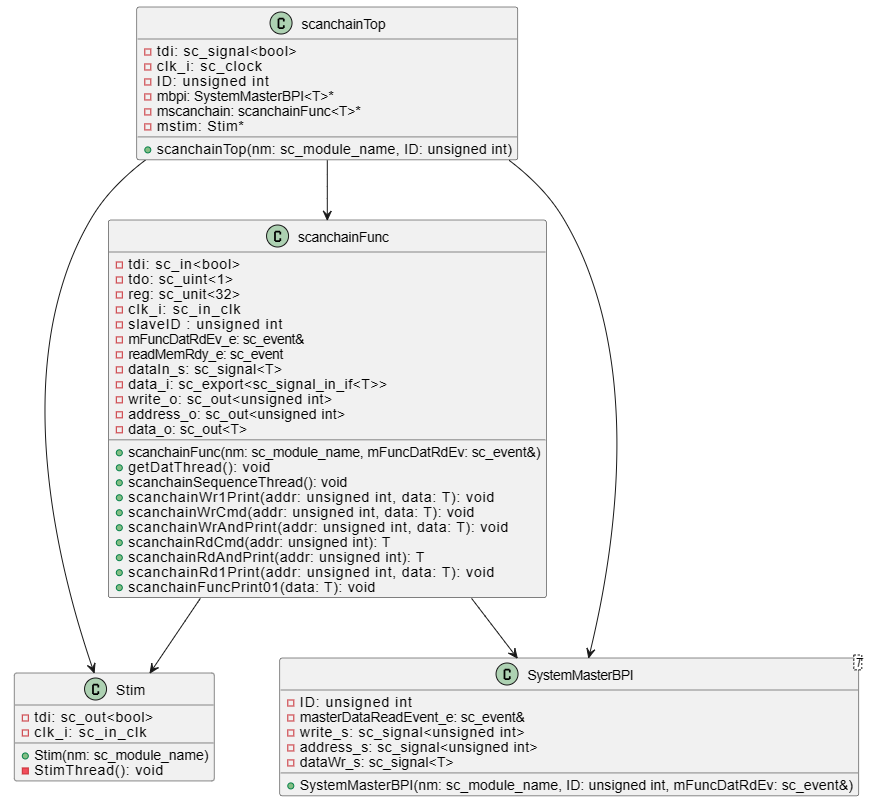
\includegraphics[width=16cm, height=18cm]{classdia.drawio.png}
  \caption{Program Logic Class Diagram}
\end{figure}



\chapter{Simulation}
\section{Module Constructors}
\begin{figure}[h!]
\centering
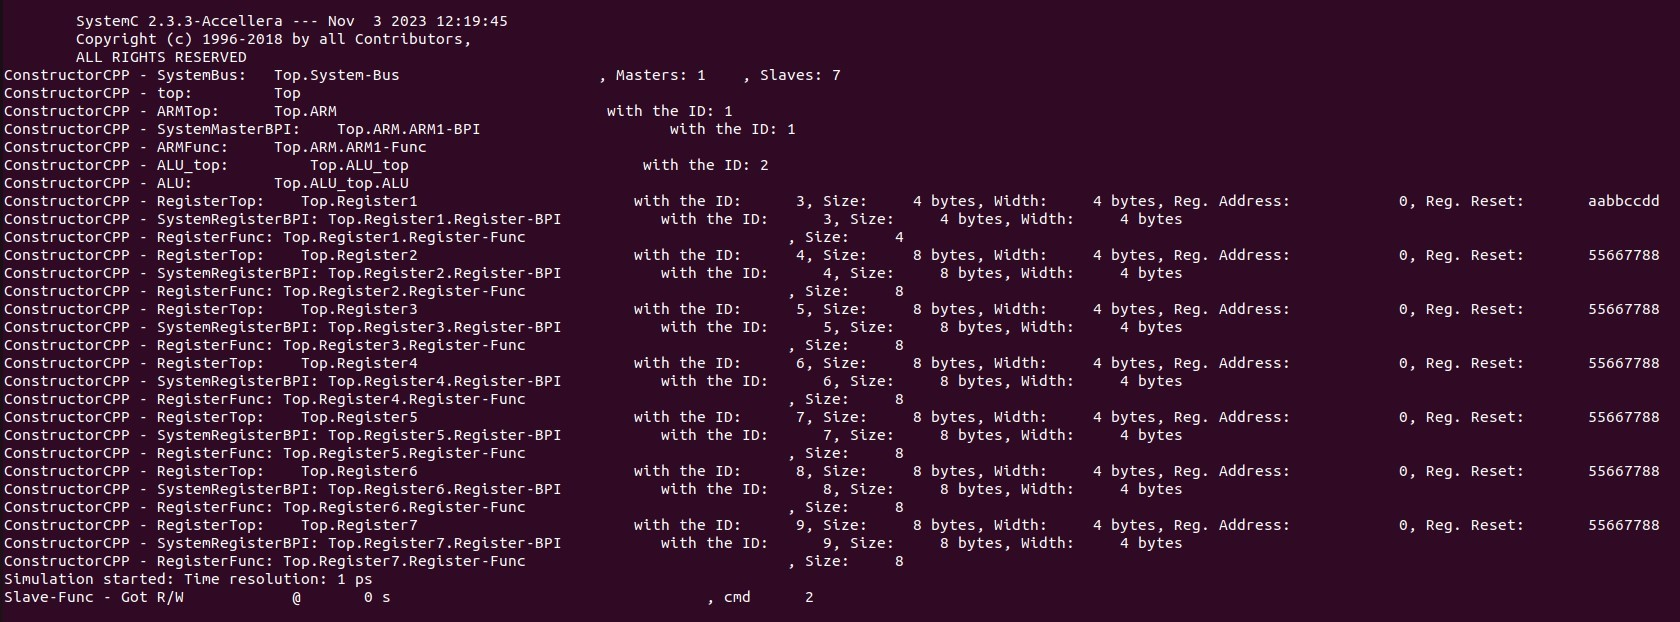
\includegraphics[width=16cm, height=10cm]{Constructor.jpg}
\caption{Constructor Prints}
\end{figure}

This provides details about module constructors seven registers instances within the system, labeled as Top.Register1 through Top.Register7. Each register is characterized by its unique identifier (ID), size, width, register address, and reset value. For instance, Register1 (Top.Register1) has an ID of 3, a size and width of 4 bytes, an address of 0, and a reset value. Similar information is provided for the other registers in the system, highlighting variations in size, width, and reset values. The log also indicates the start of the simulation with a time resolution of 1ps. Furthermore, a line in the log mentions the reception of a read/write command with a command ID of 2 by the "Slave-Func" module. This suggests that the system is interacting with external commands or stimuli, with the specific nature of this interaction depending on the system's implementation and the functionality associated with the mentioned command.

\section{Read-Write by ARM / Arithmetic Operations}
\subsection{32 Bit ALU Operations}
The two inputs, operands\_1 is 5 and operand\_2 is 4, were read from the ARM function. The AND function was then performed, yielding the desired result. Additionally, the flags operation was successfully displayed  no flag generated, as seen in the Figure\ref{ref: AND}.\\
 \begin{figure}[ht]
	\centering
	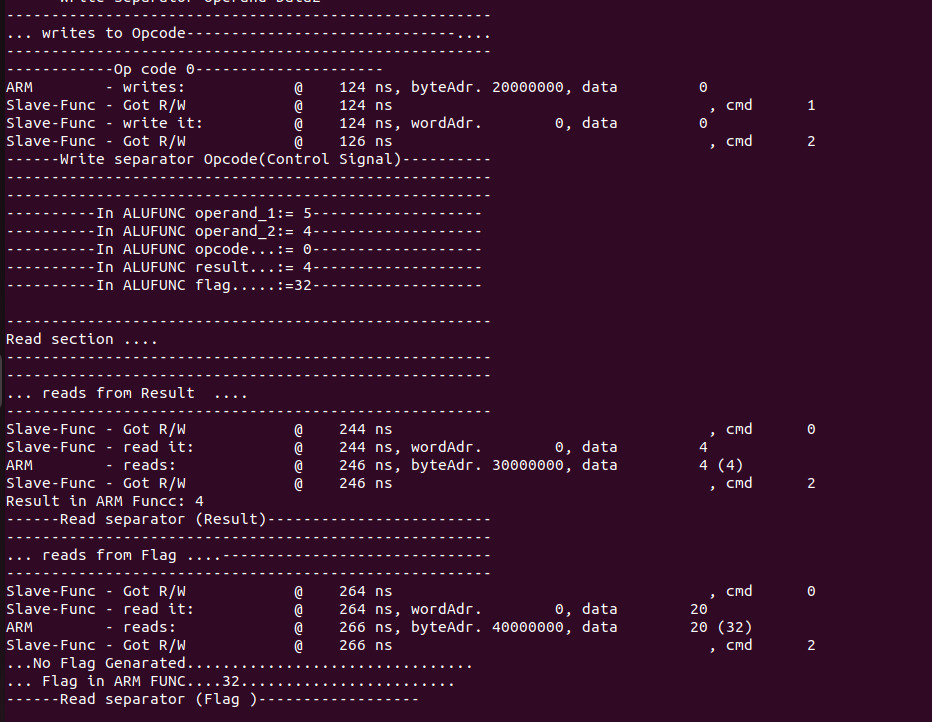
\includegraphics[width=0.9\textwidth]{AND} % Adjust the filename as needed
	\caption{The result of AND operation and the stetted flags}
	\label{ref: AND}
\end{figure}
\newpage
The operands\_1 is 1 and operands\_2 is 2 were read using the ARM function. After that, the OR function was used to get the desired result. Furthermore, the flag operations were successfully displayed. No flag was generated, as shown in Figure\ref{ref:OR}.\\
 \begin{figure}[ht]
	\centering
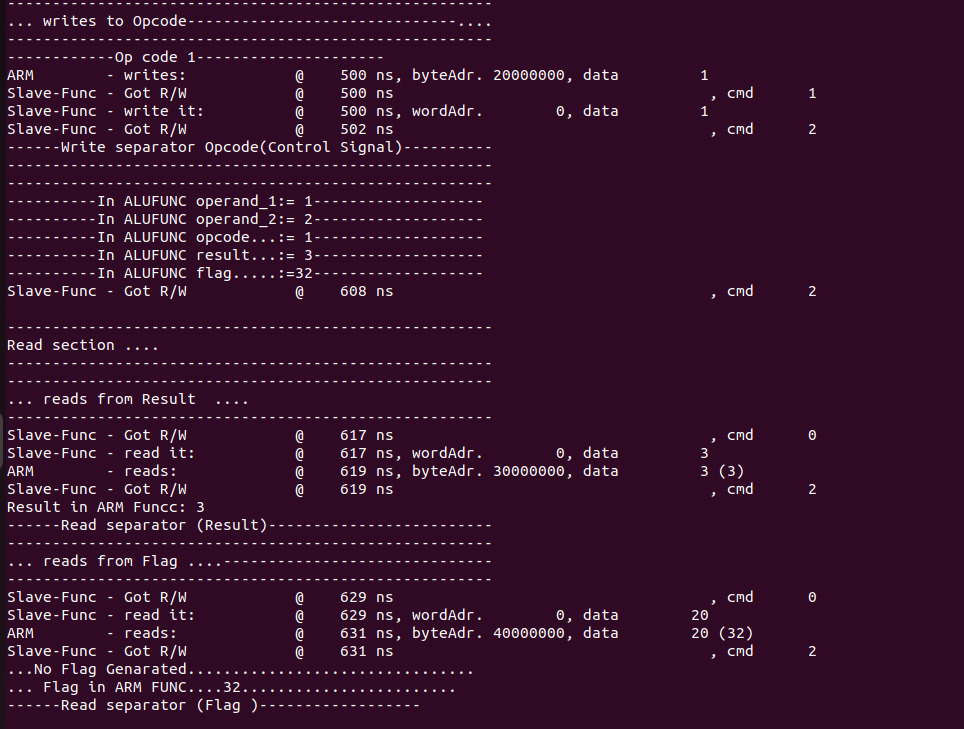
\includegraphics[width=16cm, height=10cm]{OR} % Adjust the filename as needed
	\caption{The result of OR operation and the stetted flags}
	\label{ref:OR}
\end{figure}
\newpage
The ARM function yielded the operands\_1 as 5 and operands\_2 as 6. The desired outcome was then obtained by using the addition function. In addition, as Figure\ref{ref:add} below illustrates, the flags operation—set-less than flag—was successfully displayed.\\
\begin{figure}[ht]
	\centering
	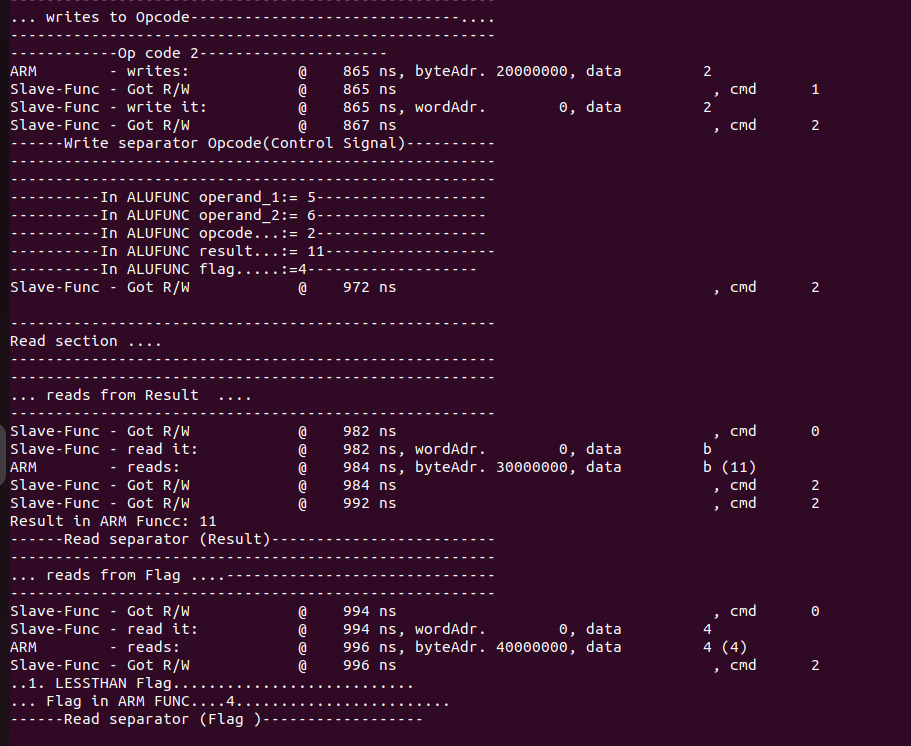
\includegraphics[width=1\textwidth]{ADD} % Adjust the filename as needed
	\caption{The result of addition operation and the stetted flags}
	\label{ref:add}
\end{figure}
\newpage
The ARM function yielded the operands\_1 as 5 and operands\_2 as 6. The desired outcome was then obtained by using the addition function. In addition, as Figure\ref{ref:add} below illustrates, the flags operation—set-less than flag—was successfully displayed.\\ operands\_1 8 and operand\_2 9 from the ARM function. After that, the subtraction function was used to get the intended result. Additionally, as Figure\ref{ref: sub} below shows, the operation of setting negative and set-less than flags was successfully displayed.\\
\begin{figure}[ht]
	\centering
	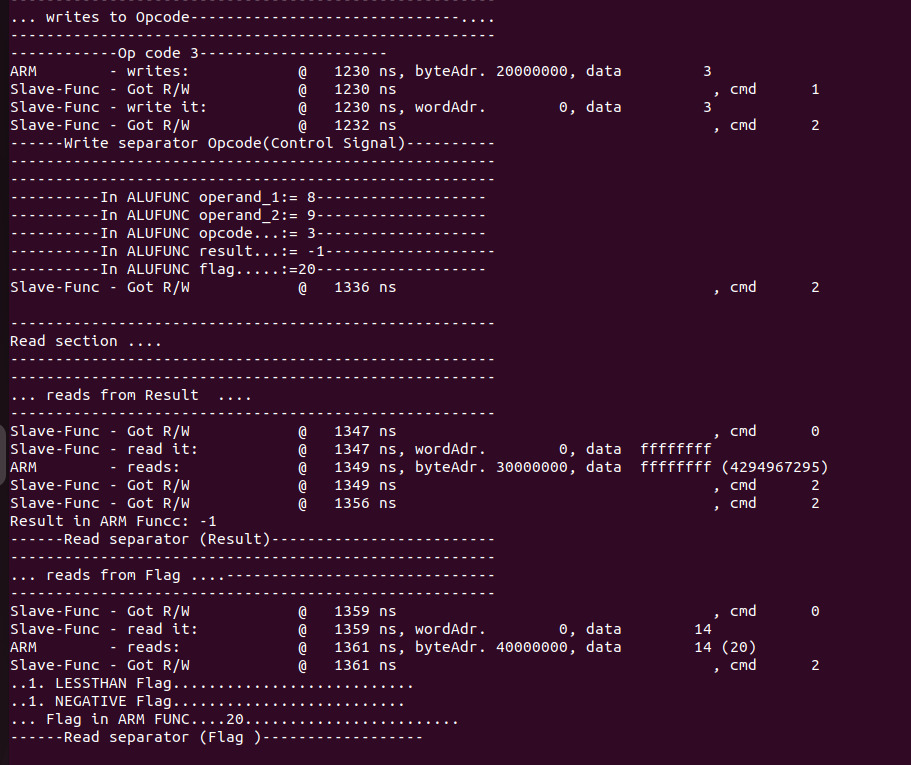
\includegraphics[width=1\textwidth]{SUB} % Adjust the filename as needed
	\caption{Flags that were displayed and the outcome of the subtraction operation}
	\label{ref: sub}
\end{figure}
\newpage
From the ARM function,  the operand\_1 as 3 and operand\_2 as 4 is obtained. After that, the desired outcome was obtained by using the set-less-than function. Furthermore, the operation of set-less than flag was successfully displayed, as shown in figure 5.6\\
\begin{figure}[ht]
	\centering
	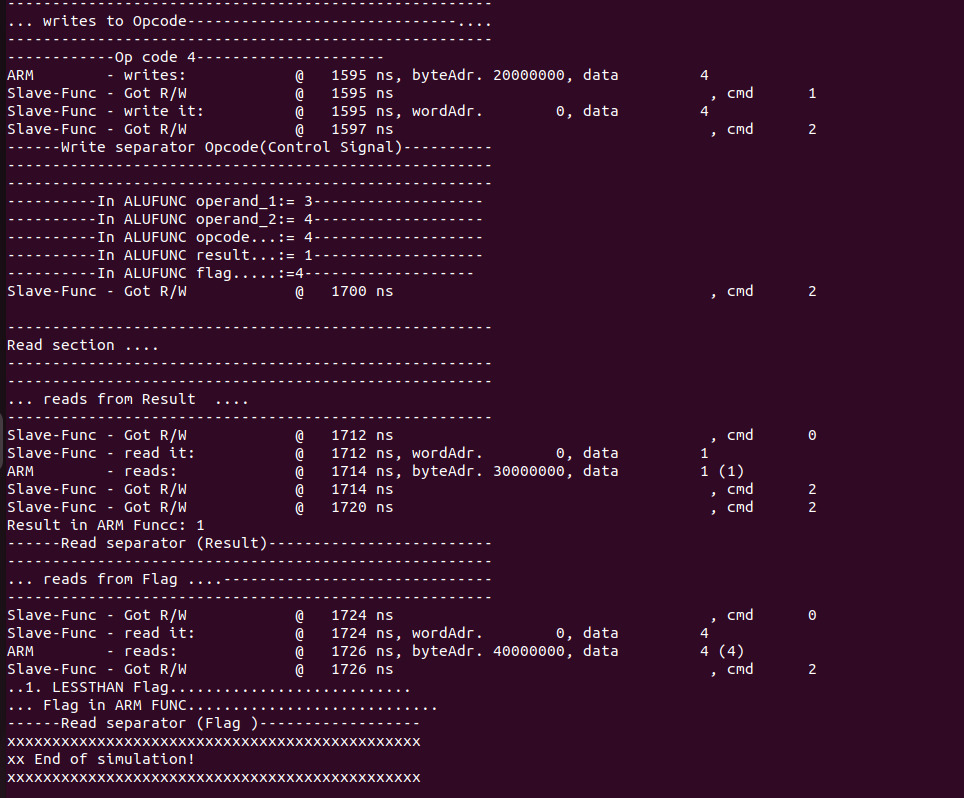
\includegraphics[width=0.9\textwidth]{lessthan} % Adjust the filename as needed
	\caption{The result of set-less-than operation and the stetted flags}
	\label{}
\end{figure}

\subsection{Test Results}

\begin{table}[h]
	\centering
	\begin{tabular}{|p{1.65cm}|p{1.65cm}|p{1.8cm}|p{3cm}|p{3cm}|}
		\hline
		Operand1 &  Operand2 &  Opcode &  Results &  Flags \\
		\hline
		5 & 4 & AND & 4 & No Flag \\
        \hline
		1 & 2 & OR & 3 & No Flag \\
        \hline
		5 & 6 & ADD & B(11) & Less Than Flag\\
        \hline
		8 & 9 & SUB & FFFFFFFF (-1) & Less Than Flag, Negative Flag \\
        \hline
		3 & 4 & COMPARE LESS THAN & Prints 1 for True & Less than Flag \\
		\hline
  
	\end{tabular}
 \caption{Test Results of ALU operations}
\end{table}
\newpage

\section{Scan Chain}
\begin{itemize}
    \item Scan chain mode or test mode is activated by enabling the Test Mode in ProcPack.h as in Figure \ref{fig:testmode}.
    \item Enabling the SLAVEFUNPRINTS and MAIN PRINTS displays the slave-func timing at each position of data communication and writing to the register along with the address and data positioning value at each shift level as shown in Figure \ref{fig:sim}.
     \item Figure \ref{fig:tdi-shift} displays the shifting of 1-bit TDI from LSB to MSB in a 32-bit Register of reg1. Once the data is shifted in each register parallely, the TDO is fetched from the MSB. The same operation occurs with the other registers.
\end{itemize}
\begin{figure}[h!]
  \centering
  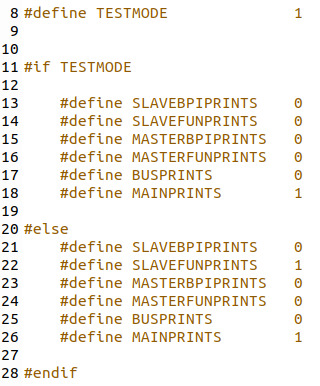
\includegraphics[width=0.3\linewidth]{testmode.jpg}
  \caption{Test Mode}
  \label{fig:testmode}
\end{figure}


\begin{figure}[h!]
  \centering
  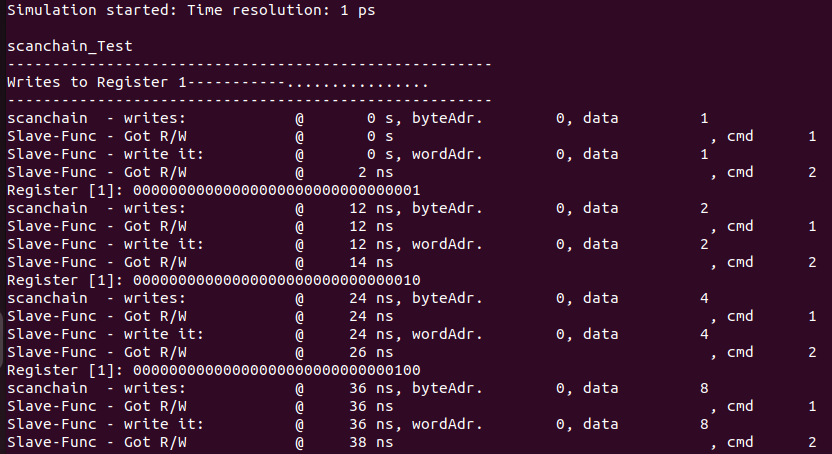
\includegraphics[width=0.7\linewidth]{Writing to reg.png}
  \caption{Simulation Output with Slave-Func}
  \label{fig:sim}
\end{figure}


\begin{figure}[h!]
  \centering
  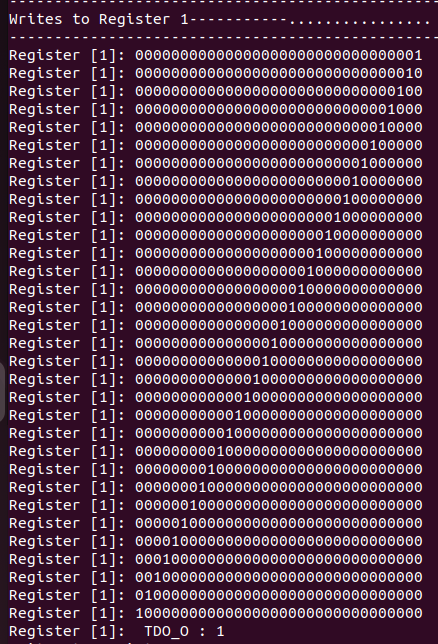
\includegraphics[width=0.7\linewidth]{reg out.png}
  \caption{Simulation Output with TDI shift}
  \label{fig:tdi-shift}
\end{figure}

\chapter{Test and Debug}
\section{Scan Chain}
\begin{itemize}
    \item Scan chain allows for the serial loading and capturing of data in a shift-register model, providing a way to observe and manipulate the internal states of the design. It involves creating a chain of flip-flops that allows for the efficient scanning of data into and out of the registers..
    \item In our design, we have implemented Scan Chain for a set of registers and captured the data via scan-in and scan-out flow parrallely to all the registers.
    \item Overall, the performance of the RISC-V ALU is good, and the expected outcome and flag status are obtained. Additionally, the status of the flags and the outcomes of arithmetic and logic operations are written back into the ARM. 
\end{itemize}
\newpage

\addcontentsline{toc}{chapter}{References} % Add reference section to the table of contents
\bibliographystyle{plain}  % You can choose a different bibliography style
\bibliography{References}  % Replace "your_bibliography_file" with the name of your .bib file

[1] Computer Organization and Design RISC-V Edition: The Hardware Software Interface. Book by David A Patterson and John L. Hennessy \newline
[2] VLSI Test Principles and Architectures. Book by Laung-Terng Wang, Cheng-Wen Wu and Xiaoqing Wen \newline
[3] IEEE Standard Test Access Port and 
Boundary-Scan Architecture (2008)
\end{enumerate}
\end{document}

